\documentclass[pdf]{beamer}

\usepackage[utf8]{inputenc}
\usepackage[T1]{fontenc}
\usepackage{graphicx}
\usepackage{tabto}
\usepackage{listings} % Required for insertion of code
\usepackage{tcolorbox}
\usepackage{subcaption}
\usepackage[main=greek, english]{babel} % For Greek language

\newcommand{\en}[1]{\foreignlanguage{english}{#1}}
\newcommand{\src}[1]{{\tt\en{#1}}}

\newcommand{\img}[1]
{
    \begin{center}
        \fcolorbox{black}{white}{\includegraphics[height=10em]{#1}}
    \end{center}

}

\beamertemplatenavigationsymbolsempty

\usetheme{Madrid}

\makeatletter
\setbeamertemplate{footline}{%
  \leavevmode%
  \hbox{%
    \begin{beamercolorbox}[wd=.35\paperwidth,ht=2.25ex,dp=1ex,center]{author in head/foot}%
      \usebeamerfont{author in head/foot}\insertshortauthor\expandafter\ifblank\expandafter{\beamer@shortinstitute}{}{~~(\insertshortinstitute)}
    \end{beamercolorbox}%
    \begin{beamercolorbox}[wd=.60\paperwidth,ht=2.25ex,dp=1ex,center]{title in head/foot}%
      \usebeamerfont{title in head/foot}\insertshorttitle
    \end{beamercolorbox}%
  }%
  \begin{beamercolorbox}[wd=.2\paperwidth,ht=2.25ex,dp=1ex,right]{date in head/foot}%
    \usebeamerfont{date in head/foot}%
    \usebeamertemplate{page number in head/foot}%
    \hspace*{2ex} 
  \end{beamercolorbox}
  \vskip0pt%
}
\makeatother

\title{Προηγμένες Τεχνικές Προγραμμτισμού - \en{Project}}
\date{}
\author{}

% \usebackgroundtemplate%
% {%
%     \includegraphics[height=\paperheight]{./template_beamer.png}%
% }

\begin{document}

\begin{frame}
    \maketitle
\end{frame}

\section{Εισαγωγή}

\begin{frame}
    \frametitle{Εφαρμοφή Υποστήριξης Κοινότητας}

    \begin{block}{Περιγραφή}
        Η εφαρμογή μας αποτελεί μία απλή υλοποίηση ενός 
        \en{forum} στο οποίο χρήστες θα μπορούν να δημιουργούν
        \en{posts}, σχόλια και να βλέπουν στατιστικά ανάλογα με τις 
        δραστηριότητές τους στην ιστοσελίδα.
    \end{block}
    
   \begin{figure}[htpb]
       \centering
        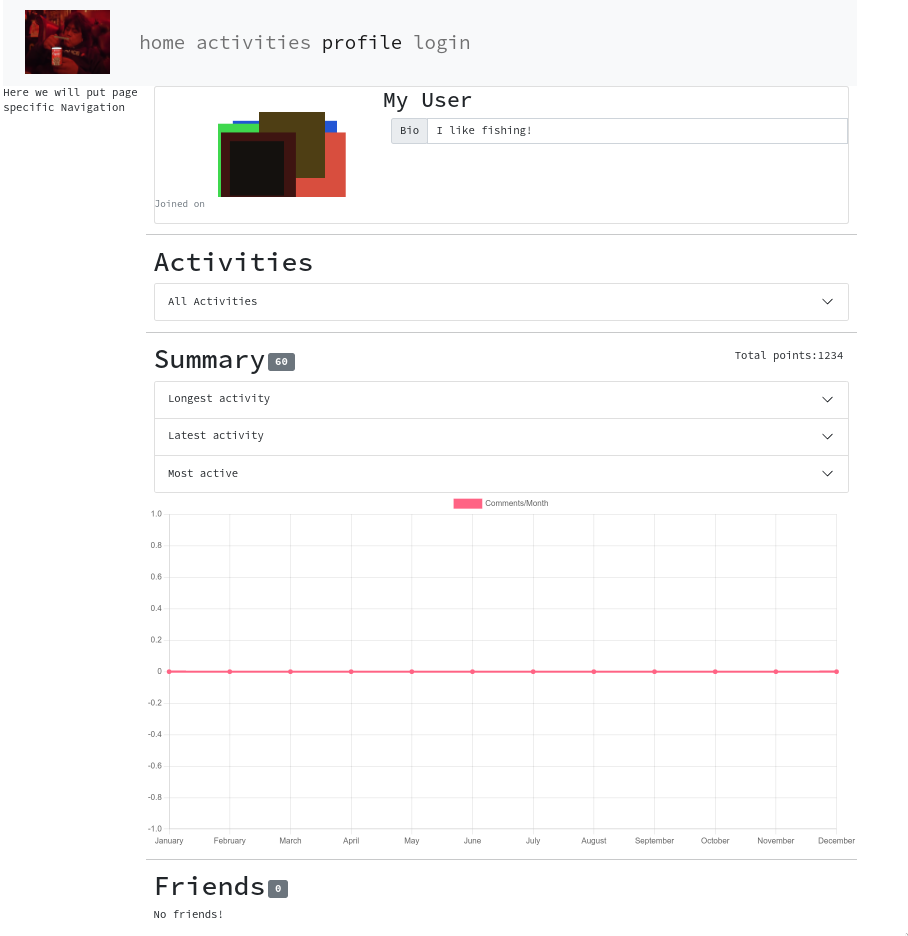
\includegraphics[width=.4\textwidth]{./assets/site.png}
   \end{figure} 
    
\end{frame}

\begin{frame}

    \frametitle{Βασικές λειτουργίες}

    \begin{itemize}
        \item Δημιουργία λογαριασμού από τον χρήστη
        \item Προσωπικό προφίλ
        \item Δημιουργία Δημοσιεύσεων / Σχόλια σε αυτές
        \item 
    \end{itemize}
    
\end{frame}


\begin{frame}
    \frametitle{\en{Tech Stack}}

\begin{figure}[htpb]
    \centering

    \smartdiagram[descriptive diagram]{
        {\en{Bootstrap}, {Έτοιμα \src{CSS/Javascript} \en{components}}},
        {\en{Handlebars}, {\src{HTML} \en{Render Engine}}},
        {\en{Express}, {\en{WebServer}}},
        {\en{Node}, {Περιβάλλον εκτέλεσης \src{Javascript}}},
        {\en{MySQL/SQLite}, {\en{DataBase Management System}}},
}
    \caption{Τα βάσικα μερή του \en{technology stack} που χρησιμοποιήσαμε.}
\end{figure}

\end{frame}


\end{document}
